\documentclass[11pt,aspectratio=169]{beamer}
\usepackage[utf8]{inputenc}
\usepackage[T1]{fontenc}
\usepackage{graphicx}
\usepackage{booktabs}
\usepackage{xcolor}
\usepackage{tikz}

\usetheme{Madrid}
\usecolortheme{whale}

\definecolor{myblue}{RGB}{15,60,120}
\definecolor{myred}{RGB}{231,76,60}
\definecolor{mygreen}{RGB}{46,204,113}
\definecolor{myorange}{RGB}{243,156,18}
\definecolor{mypurple}{RGB}{155,89,182}
\definecolor{mygold}{RGB}{255,215,0}

\setbeamercolor{title}{fg=white,bg=myblue}
\setbeamercolor{frametitle}{fg=white,bg=myblue}
\setbeamercolor{structure}{fg=myblue}

\title[Optimización de Rutas -- Chachapoyas]{Optimización de Rutas de Recolección\\de Residuos Sólidos en Chachapoyas, Perú}
\subtitle{Análisis Comparativo de 5 Algoritmos de Ruteo sobre Grafos Viales}
\author{Proyecto de Investigación -- Diseño y Análisis de Algoritmos}
\date{Julio 2026}

\begin{document}

% ===== SLIDE 1: TITLE =====
\begin{frame}
\titlepage
\end{frame}

% ===== SLIDE 2: CONTEXT =====
\begin{frame}{Contexto y Motivación}
\begin{columns}[T]
\column{0.55\textwidth}
\textbf{Chachapoyas, Amazonas, Perú}
\begin{itemize}
  \item Capital del departamento de Amazonas
  \item 2,335 m s.n.m. en la cordillera de los Andes
  \item Trazado urbano colonial irregular
  \item Calles estrechas de un solo sentido
  \item Crecimiento orgánico no planificado
\end{itemize}

\vspace{8pt}
\textbf{Problema operativo}
\begin{itemize}
  \item 60--80\% del presupuesto de limpieza se gasta en recolección y transporte
  \item Flota de 5 camiones recolectores
  \item 111.27 km de calles a servir
\end{itemize}

\column{0.45\textwidth}
\centering
\textbf{Objetivo}\\
\smallskip
Encontrar el algoritmo de ruteo más eficiente para minimizar la distancia total recorrida, manteniendo cobertura completa.
\bigskip

\begin{block}{Pregunta de investigación}
¿Qué enfoque algorítmico minimiza la distancia total recorrida por la flota de recolección en Chachapoyas?
\end{block}
\end{columns}
\end{frame}

% ===== SLIDE 3: METHODOLOGY OVERVIEW =====
\begin{frame}{Metodología: Pipeline Completo}
\begin{center}
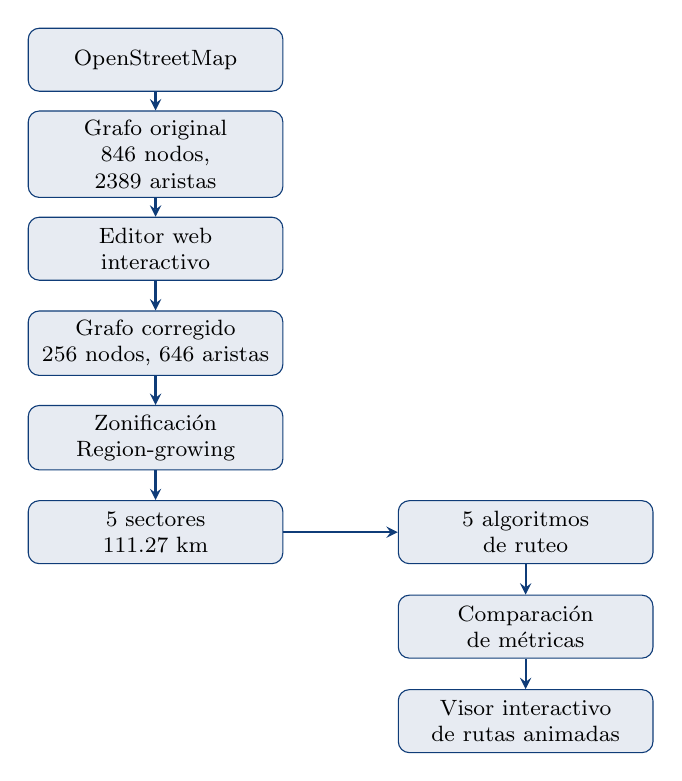
\begin{tikzpicture}[node distance=1.2cm, auto,
  block/.style={rectangle, draw=myblue, fill=myblue!10, text width=3cm, text centered, rounded corners, minimum height=0.8cm, font=\footnotesize},
  arrow/.style={->, >=stealth, thick, myblue}]

\node[block] (osm) {OpenStreetMap};
\node[block, below of=osm] (graph) {Grafo original\\846 nodos, 2389 aristas};
\node[block, below of=graph] (editor) {Editor web\\interactivo};
\node[block, below of=editor] (corrected) {Grafo corregido\\256 nodos, 646 aristas};
\node[block, below of=corrected] (zoning) {Zonificación\\Region-growing};
\node[block, below of=zoning] (sectors) {5 sectores\\111.27 km};
\node[block, right of=sectors, xshift=3.5cm] (algorithms) {5 algoritmos\\de ruteo};
\node[block, below of=algorithms] (results) {Comparación\\de métricas};
\node[block, below of=results] (visor) {Visor interactivo\\de rutas animadas};

\draw[arrow] (osm) -- (graph);
\draw[arrow] (graph) -- (editor);
\draw[arrow] (editor) -- (corrected);
\draw[arrow] (corrected) -- (zoning);
\draw[arrow] (zoning) -- (sectors);
\draw[arrow] (sectors) -- (algorithms);
\draw[arrow] (algorithms) -- (results);
\draw[arrow] (results) -- (visor);
\end{tikzpicture}
\end{center}
\end{frame}

% ===== SLIDE 4: GRAPH =====
\begin{frame}{Grafo Vial}
\begin{columns}[T]
\column{0.5\textwidth}
\textbf{Construcción}
\begin{itemize}
  \item Descarga OSMnx, radio 3 km
  \item Tipo \texttt{drive}, simplificación automática
  \item \texttt{networkx.MultiDiGraph}
  \item Peso de arista = distancia (m)
\end{itemize}

\vspace{8pt}
\textbf{Corrección manual}
\begin{itemize}
  \item Editor web (Leaflet.js + Python HTTP)
  \item CRUD nodos/aristas, drag \& drop
  \item Puntos de control, direcciones
  \item Simplificación, restauración
  \item 846 nodos $\rightarrow$ 256 nodos
\end{itemize}

\column{0.5\textwidth}
\textbf{Exclusiones}
\begin{itemize}
  \item 4 nodos excluidos (depósito, conector, acceso)
  \item 3 aristas de ruta al depósito (7.21 km)
  \item 111.27 km efectivos de servicio
\end{itemize}

\vspace{8pt}
\textbf{Nodo depósito}
\begin{itemize}
  \item \texttt{af3202cd-3a9f\ldots}
  \item Todas las rutas inician y terminan aquí
\end{itemize}
\end{columns}
\end{frame}

% ===== SLIDE 5: ZONING =====
\begin{frame}{Zonificación: Region-Growing}
\begin{columns}[T]
\column{0.55\textwidth}
\textbf{Region-growing sobre el grafo}
\begin{enumerate}
  \item 5 semillas geográficas (4 esquinas + centro)
  \item BFS simultánea desde todas las semillas
  \item Cada sector para al alcanzar $\sim$22 km
  \item Post-balanceo + reparación conectividad
\end{enumerate}

\vspace{8pt}
\textbf{Ventajas sobre K-Means}
\begin{itemize}
  \item Garantiza conectividad por construcción
  \item Sin ajustes manuales
  \item Balance 1.16x (K-Means: 1.68x)
  \item Balance tiempo DCPP 1.11x (K-Means: 3.39x)
\end{itemize}

\column{0.45\textwidth}
\centering
\textbf{Distribución final}\\[4pt]
\begin{tabular}{cccc}
\toprule
\textbf{S} & \textbf{Nodos} & \textbf{Aristas} & \textbf{km}\\
\midrule
\rowcolor{myred!15}    S0 & 36 & 91  & 20.54\\
\rowcolor{myblue!15}   S1 & 33 & 90  & 22.50\\
\rowcolor{mygreen!15}  S2 & 39 & 107 & 23.33\\
\rowcolor{myorange!15} S3 & 51 & 137 & 22.12\\
\rowcolor{mypurple!15} S4 & 93 & 215 & 22.78\\
\midrule
\textbf{Total} & 252 & 640 & 111.27\\
\bottomrule
\end{tabular}

\vspace{6pt}
\tiny Balance: max/min = 1.16x
\end{columns}
\end{frame}

% ===== SLIDE 6: ALGORITHMS =====
\begin{frame}{Algoritmos de Ruteo}
\begin{columns}[T]
\column{0.33\textwidth}
\textbf{Voraz}
\begin{itemize}
  \item Línea base
  \item Siempre a la arista no servida más cercana
  \item Dijkstra con caché
  \item O(n·(E+V log V))
  \item \textcolor{red}{Redundancia alta}
\end{itemize}

\column{0.33\textwidth}
\textbf{DCPP}
\begin{itemize}
  \item Cartero Chino Dirigido
  \item Húngaro (O(m³)) para balanceo de grados
  \item Hierholzer para circuito Euleriano
  \item Soporte multi-componente
  \item \textcolor{mygreen}{Óptimo para CPP}
\end{itemize}

\column{0.33\textwidth}
\textbf{CARP-Ulusoy ★}
\begin{itemize}
  \item Route-first-cluster-second
  \item Hereda orden del circuito DCPP
  \item Conecta aristas por camino más corto
  \item Evita deadhead de aristas fantasma
  \item \textcolor{mygold}{\textbf{Mejor resultado}}
\end{itemize}
\end{columns}

\vspace{12pt}
\begin{columns}[T]
\column{0.5\textwidth}
\textbf{CARP + Tabú}
\begin{itemize}
  \item Capacidad 30 km/viaje (no vinculante aquí)
  \item 2-opt + relocate, 150 iteraciones
  \item Mejora marginal respecto al Voraz
\end{itemize}

\column{0.5\textwidth}
\textbf{MCPP (validación)}
\begin{itemize}
  \item Modelo no dirigido de referencia
  \item Calles doble sentido = 1 pasada
  \item Matching de nodos impares
  \item \textit{Valida que el modelo dirigido no sesga}
\end{itemize}
\end{columns}
\end{frame}

% ===== SLIDE 7: KEY INSIGHT =====
\begin{frame}{Hallazgo Clave: ¿Por qué Ulusoy supera al DCPP?}
\begin{center}
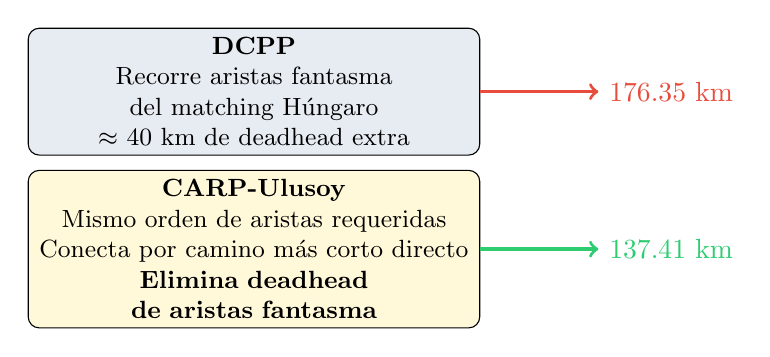
\begin{tikzpicture}[node distance=2cm, auto,
  block/.style={rectangle, draw, text width=5.5cm, text centered, rounded corners, minimum height=1.5cm, font=\small}]

\node[block, fill=myblue!10] (dcpp) {\textbf{DCPP}\\
Recorre aristas fantasma del matching Húngaro\\
$\approx$ 40 km de deadhead extra};

\node[block, fill=mygold!15, below of=dcpp] (ulusoy) {\textbf{CARP-Ulusoy}\\
Mismo orden de aristas requeridas\\
Conecta por camino más corto directo\\
\textbf{Elimina deadhead de aristas fantasma}};

\draw[->, very thick, myred] (dcpp.east) -- ++(1.5,0) node[right] {176.35 km};
\draw[->, very thick, mygreen] (ulusoy.east) -- ++(1.5,0) node[right] {137.41 km};
\end{tikzpicture}
\end{center}

\vspace{12pt}
\begin{block}{Condiciones de comparación justa}
\begin{itemize}
  \item Mismo grafo $G_u$ para medir distancias
  \item Sin penalizaciones artificiales en deadhead
  \item Todos los algoritmos usan la misma métrica
\end{itemize}
\end{block}
\end{frame}

% ===== SLIDE 8: RESULTS TABLE =====
\begin{frame}{Resultados: Comparativa de 5 Algoritmos}
\begin{table}
\centering
\footnotesize
\begin{tabular}{lcccccc}
\toprule
\textbf{S} & \textbf{Algoritmo} & \textbf{Dist (km)} & \textbf{Serv (km)} & \textbf{Redund} & \textbf{Tiempo (h)} & \textbf{CPU (s)}\\
\midrule
\rowcolor{myred!10}    0 & Voraz      & 41.96 & 20.54 & 2.043 & 8.39 & 0.048\\
\rowcolor{myred!10}    0 & DCPP       & 34.20 & 20.54 & 1.665 & 6.84 & 0.020\\
\rowcolor{myred!10}    0 & CARP+Tabu  & 39.68 & 20.54 & 1.932 & 7.94 & 0.348\\
\rowcolor{myred!10}    0 & \textbf{CARP-Ulusoy} & \textbf{26.84} & 20.54 & 1.307 & 5.37 & 0.055\\
\addlinespace
\rowcolor{myblue!10}   1 & Voraz      & 39.09 & 22.50 & 1.738 & 7.82 & 0.048\\
\rowcolor{myblue!10}   1 & DCPP       & 33.80 & 22.50 & 1.502 & 6.76 & 0.021\\
\rowcolor{myblue!10}   1 & \textbf{CARP-Ulusoy} & \textbf{27.53} & 22.50 & 1.224 & 5.51 & 0.045\\
\addlinespace
\rowcolor{mygreen!10}  2 & Voraz      & 44.17 & 23.33 & 1.893 & 8.83 & 0.061\\
\rowcolor{mygreen!10}  2 & \textbf{CARP-Ulusoy} & \textbf{27.64} & 23.33 & 1.185 & 5.53 & 0.053\\
\addlinespace
\rowcolor{myorange!10} 3 & Voraz      & 41.30 & 22.12 & 1.867 & 8.26 & 0.067\\
\rowcolor{myorange!10} 3 & \textbf{CARP-Ulusoy} & \textbf{28.10} & 22.12 & 1.270 & 5.62 & 0.062\\
\addlinespace
\rowcolor{mypurple!10} 4 & Voraz      & 44.99 & 22.78 & 1.975 & 9.00 & 0.099\\
\rowcolor{mypurple!10} 4 & \textbf{CARP-Ulusoy} & \textbf{27.29} & 22.78 & 1.198 & 5.46 & 0.104\\
\bottomrule
\end{tabular}
\end{table}

\vspace{-6pt}
\begin{table}
\centering
\small
\begin{tabular}{lcccc}
\toprule
\textbf{Algoritmo} & \textbf{Total (km)} & \textbf{Redund} & \textbf{Tiempo (h)} & \textbf{CPU (s)}\\
\midrule
Voraz      & 211.51 & 1.903 & 42.30 & 0.323\\
DCPP       & 176.35 & 1.587 & 35.27 & 0.111\\
CARP+Tabu  & 206.61 & 1.858 & 41.32 & 2.508\\
\textbf{CARP-Ulusoy} & \textbf{137.41} & \textbf{1.237} & \textbf{27.48} & 0.318\\
MCPP       & 178.51 & 2.690 & 35.70 & 0.160\\
\bottomrule
\end{tabular}
\end{table}
\end{frame}

% ===== SLIDE 9: CHART =====
\begin{frame}{Mejora Relativa sobre la Línea Base}
\begin{center}
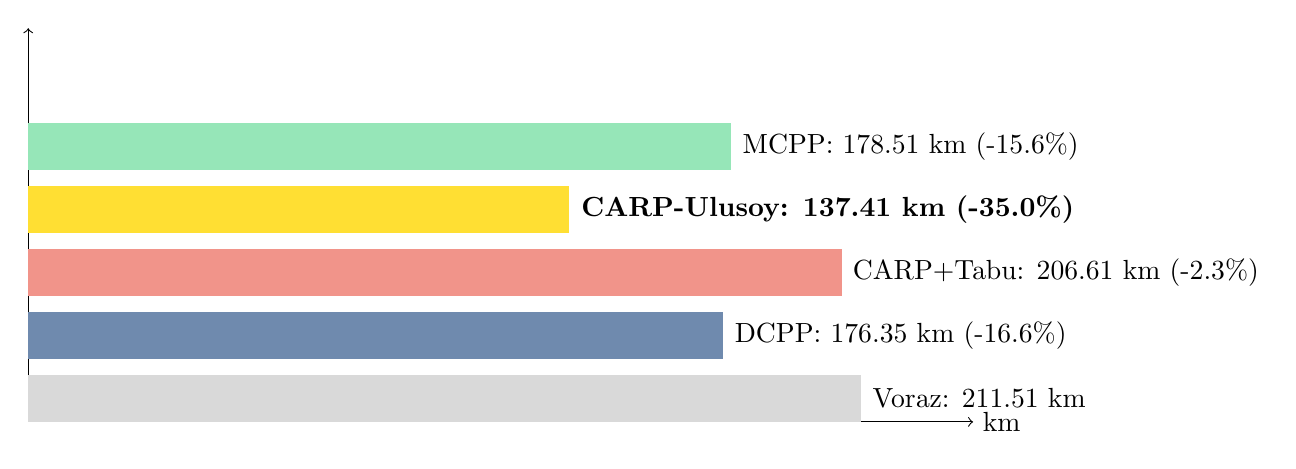
\begin{tikzpicture}
\draw[->] (0,0) -- (12,0) node[right] {km};
\draw[->] (0,0) -- (0,5);

% Voraz baseline bar (100%)
\fill[gray!30] (0,0) rectangle (10.58,0.6);
\node[anchor=west] at (10.6,0.3) {Voraz: 211.51 km};

% DCPP
\fill[myblue!60] (0,0.8) rectangle (8.82,1.4);
\node[anchor=west] at (8.85,1.1) {DCPP: 176.35 km (-16.6\%)};

% CARP+Tabu
\fill[myred!60] (0,1.6) rectangle (10.33,2.2);
\node[anchor=west] at (10.35,1.9) {CARP+Tabu: 206.61 km (-2.3\%)};

% CARP-Ulusoy
\fill[mygold!80] (0,2.4) rectangle (6.87,3.0);
\node[anchor=west] at (6.9,2.7) {\textbf{CARP-Ulusoy: 137.41 km (-35.0\%)}};

% MCPP
\fill[mygreen!50] (0,3.2) rectangle (8.93,3.8);
\node[anchor=west] at (8.95,3.5) {MCPP: 178.51 km (-15.6\%)};

\end{tikzpicture}
\end{center}

\vspace{8pt}
\begin{center}
\large\textbf{CARP-Ulusoy reduce la distancia total en 74.10 km}\\
\textbf{respecto a la línea base Voraz.}
\end{center}
\end{frame}

% ===== SLIDE 10: TOOLS =====
\begin{frame}{Ecosistema de Herramientas}
\begin{columns}[T]
\column{0.33\textwidth}
\textbf{Editor Vial}\\
\texttt{editor\_grafo\_\ldots.py}
\begin{itemize}
  \item Servidor web live
  \item Leaflet.js interactivo
  \item CRUD completo de grafo
  \item Backup automático
\end{itemize}

\column{0.33\textwidth}
\textbf{Visor de Sectores}\\
\texttt{visor\_live\_sectores.py}
\begin{itemize}
  \item Mapa coloreado por sector
  \item Toggle mostrar/ocultar
  \item Click para metadatos
  \item API de datos en vivo
\end{itemize}

\column{0.33\textwidth}
\textbf{Visor de Rutas}\\
\texttt{visor\_rutas\_anim.py}
\begin{itemize}
  \item 5 sectores $\times$ 4 algoritmos
  \item Animación con estela dorada
  \item Selector sector/algoritmo
  \item Retorno al depósito
  \item Play/Pause/Velocidad
\end{itemize}
\end{columns}

\vspace{12pt}
\begin{center}
\textbf{+}\quad
\texttt{main.py} (orquestador)\quad$\cdot$\quad
\texttt{\_data.py} (datos compartidos)\quad$\cdot$\quad
\texttt{dijkstra.py} (implementación propia)
\end{center}
\end{frame}

% ===== SLIDE 11: VALIDATION =====
\begin{frame}{Validación del Modelo}
\begin{columns}[T]
\column{0.5\textwidth}
\textbf{MCPP: Validación del modelo dirigido}
\begin{itemize}
  \item Hipótesis: ¿el modelo dirigido infla distancias al forzar 2 pasadas en calles doble sentido?
  \item Resultado: NO
  \item DCPP = 176.35 km vs MCPP = 178.51 km
  \item Diferencia: apenas 1.2\%
  \item El matching de grados del DCPP compensa el servicio extra
\end{itemize}

\column{0.5\textwidth}
\textbf{Rigor estadístico}
\begin{itemize}
  \item CARP+Tabu: 10 corridas con semillas distintas
  \item Media: 206.63 $\pm$ 1.03 km
  \item Baja variabilidad confirma estabilidad del bajo rendimiento
  \item Voraz y DCPP son determinísticos
  \item CARP-Ulusoy usa semilla fija en Húngaro
\end{itemize}
\end{columns}

\vspace{12pt}
\begin{block}{Hallazgo}
El modelo dirigido (DCPP) \textbf{no infla} la distancia total. La reducción en deadhead del matching dirigido compensa exactamente el kilometraje adicional de servicio en calles de doble sentido.
\end{block}
\end{frame}

% ===== SLIDE 12: CONCLUSIONS =====
\begin{frame}{Conclusiones}
\begin{enumerate}
  \item \textbf{CARP-Ulusoy es el mejor algoritmo} para Chachapoyas: 137.41 km totales, 35.0\% mejor que Voraz, 22.1\% mejor que DCPP.
  \bigskip
  \item \textbf{Region-growing} produce sectores balanceados (1.16x) y conexos, eliminando ajustes manuales y reparación post-hoc.
  \bigskip
  \item \textbf{La capacidad de 30 km no es vinculante} con sectores balanceados ($\sim$22 km c/u). Un solo viaje por sector es suficiente.
  \bigskip
  \item \textbf{El modelo dirigido es válido}: DCPP $\approx$ MCPP (176.35 vs 178.51 km). No introduce sesgo.
  \bigskip
  \item \textbf{Metodología reproducible}: código abierto, herramientas interactivas, métrica unificada.
\end{enumerate}
\end{frame}

% ===== SLIDE 13: FUTURE WORK =====
\begin{frame}{Trabajo Futuro}
\begin{columns}[T]
\column{0.5\textwidth}
\textbf{Corto plazo}
\begin{itemize}
  \item Validación contra benchmarks estándar (mval, egl)
  \item Datos reales de elevación para modelar pendientes
  \item Múltiples depósitos / puntos de descarga
  \item Ajuste dinámico por llenado de contenedores (IoT)
\end{itemize}

\column{0.5\textwidth}
\textbf{Largo plazo}
\begin{itemize}
  \item Generalización a otras ciudades latinoamericanas
  \item Optimización multi-objetivo (distancia + emisiones + balance)
  \item Integración con sistemas GIS municipales
  \item Publicación en revista indexada
\end{itemize}
\end{columns}

\vspace{16pt}
\begin{center}
\large\textbf{Repositorio:} \texttt{github.com/elable947/garbage\_proj}\\[4pt]
Rama \texttt{mejoras} -- todas las mejoras implementadas
\end{center}
\end{frame}

% ===== SLIDE 14: THANKS =====
\begin{frame}[plain]
\begin{center}
\Huge\textcolor{myblue}{¡Gracias!}\\[16pt]
\Large ¿Preguntas?\\[24pt]
\normalsize
\texttt{github.com/elable947/garbage\_proj}
\end{center}
\end{frame}

\end{document}
